\chapter{Experimenteller Aufbau}
\begin{figure}[H]
    \centering
    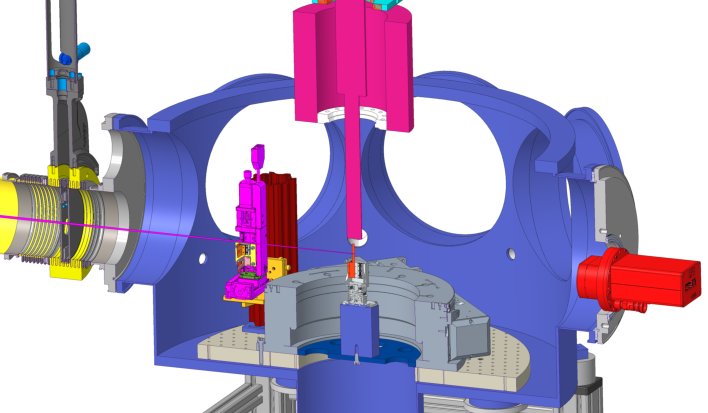
\includegraphics{images/aufbau/aufbau_empty.pdf}
    \caption{Die Skizze des Anlageaufbaus. Die Einzelbauteile sind farbig kodiert. In der Vakuumkammer (blau) wird der Druck in Höhe von ca. \SI{2.4e6}{\milli\bar} aufrechterhaltet. Der Probehalter (pink) ist aus Kupfer gemacht und kann die Rolle eines Wärmeleiters für die Probenkühlung spielen. Dazu ist der Probehalter mit der Kryoanlage angeschlossen. Der Probehalter lässt sich in. Der horizontale Spalt (fuchsia) dient zum Abschneiden des gewünschten Stahlsanduhrbereichs. Die Spaltlage sowie die Spaltbreite kann beliebig verstellt werden. Der MÖNCH-Detektor (rot) ist an der zum Strahlgang (gelb) gegenüberliegenden Wand der Vakuumkammer befestigt.}
    \label{fig:anlage}
\end{figure}